\documentclass[journal]{IEEEtran}

  \usepackage{natbib}
  \usepackage[pdftex]{graphicx}
  \usepackage[justification=centering]{caption}
  
  \DeclareGraphicsExtensions{.png}

\hyphenation{op-tical net-works semi-conduc-tor}


\begin{document}
  
\title{An Infrastructure for Automatic Installation of Applications Based on the User's Current Location}

\author{
        Bruno G. Ferreira,
        Durval P. C. Neto,
        Leandro M. de Sales,
        Thiago B. M. de Sales
}

\maketitle

\begin{abstract}
This paper presents a context-aware middleware that allows automatic installation of useful  applications on user's mobile devices based on their current locations.
\end{abstract}

\IEEEpeerreviewmaketitle

\section{Introduction}

\IEEEPARstart{B}{ased} on the term of Ubiquitous Computing, Mark Weiser envisioned a world where computing is embedded into our everyday devices, providing useful services to  users without requiring much effort or technical knowledges~\cite{weiser1991computer}. However, nowadays, the distribution of mobile applications is centralized in virtual stores, which means that users need to access a virtual store, search for the applications and then select the desired one for downloading. When the download is finished, the user needs to install the application, which also requires user's authorization in order to application get access to the phone's main hardware features, such as camera, microphone and bluetooth. The Mark's goal is hard to achieve since it is still required much effort from the users to download the application from the store, rather then get it automatically installed when needed. Therefore, in this paper, we propose a middleware that allows self-installable applications based on the services available on the users' everyday environments. The middleware is based on the Universal Plug and Play (UPnP) standards and provides two main modules: the BRisa Central Apps (BCA) and the BRisa Central User (BCU), which are detailed in the next section.

\section{Architecture}

The BCU module is a UPnP Control Point that searches for BCA devices in the network. On the other hand, BCA is a UPnP Device that provides applications to BCU. The BCA is installed on a computer in the environments where the applications will be available. The BCU is installed on the users' mobile devices, allowing them to automatically receive the available applications.

The protocol that manages all the communications among BCAs and BCUs is called BRisa Apps Communication Protocol (BACP). The architecture offers a peer-to-peer pervasive network connectivity among all types of devices, including laptops and desktops. The communication process between the BCU and the BCA is summarized in Fig. 1. In Step 1, when the BCU enters into a new environment and connects to the local network, it sends a UPnP SSDP (Service Discovery Protocol) request to discover BCA devices. In Step 2, upon receiving the BCU's discovery message, one or more BCA devices reply to the BCU by sending a message that contains important information about the BCA device and other information regarding its services, which allows the BCU to install the available applications. In Step 3, the BCU sends a request to each BCA device available in the local network, asking for the name and icon of each application available in BCA. Once the BCU receives such data from the BCA (Step 4), each application icon is exposed on the applications menu of the BCU(Step 5). In Step 6, if the user is interested in any of the applications that has been shown on the screen, (s)he can select its icon. In Step 7, the BCU sends a request to the respective BCA in order to download the files needed. In Step 8, these files are downloaded in a compressed format and extracted on the BCU. The main application file is then executed on user's BCU(Step 9). When the user leaves the environment, the application is automatically removed, freeing up storage space on the device.

\begin{figure}[tb]
    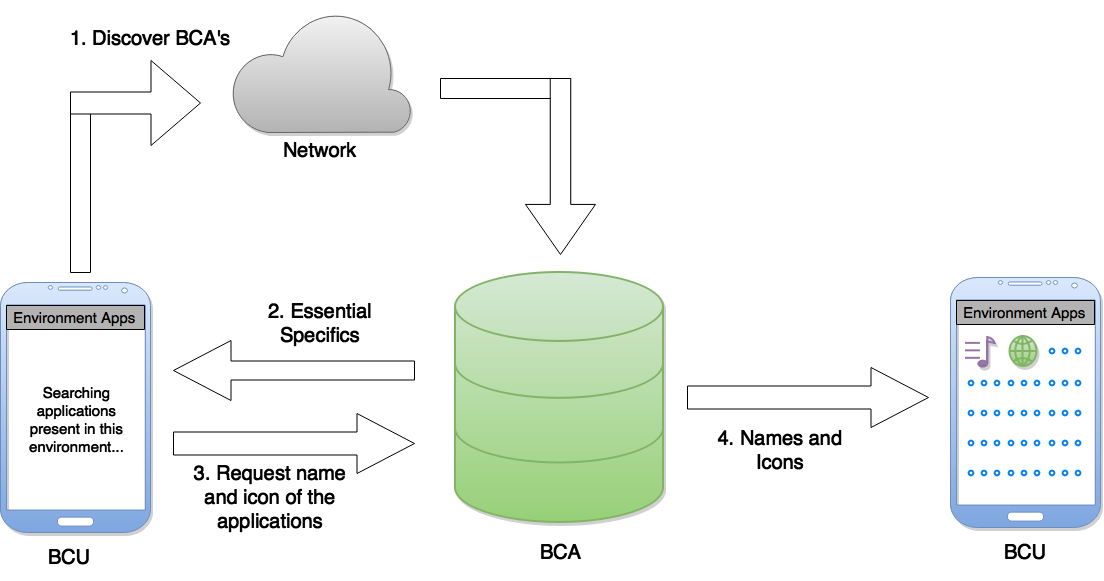
\includegraphics[scale = 0.36]{FIG1}    
    \caption{Brief communication between BCU and BCA devices.}
\end{figure}

Optionally, the user can activate a caching mechanism to avoid downloading applications that were previously executed. However, before the client eventually executes the application stored in the cache, the client module checks if a newer version of the application is available in the BCA device that hosts the application. So, the BCU executes the BRisa Application Communication Protocol (BACP). The details of such communication  is depicted in Fig. 2.

The BCA device was developed with the BRisa framework ~\cite{guedes2008brisa}, which is developed in Qt/QML Language, a subset of the Qt Framework. Qt is a multiparadigm language for creating highly dynamic applications. The format of an application is a set of QML files along with other resources used by the QML files. To host an application on the BCA, the files must be installed in a specific folder presented on the BCA. The directory structure of a BCA that hosts two applications is depicted in Fig. 3. When the BCA sends the list of available applications to the BCU, it transfers a JSON file along with the applications' names and icons' URLs. When the user chooses which application will be executed by selecting the icon of the application, the BCA sends a JSON content with the application's title, the icon's URL, a short application description and all the services that the application exposes to BCU. If the user get interested in the application, BCA will send a JSON content with a URL of the main QML of the application. 

\section{Description of a Case Study}
Suppose a scenario where a user arrives at a Shopping mall. The mall provides an application which icon's is automatically displayed on the main menu of the user's BCU device.

\begin{figure}[!htb]
    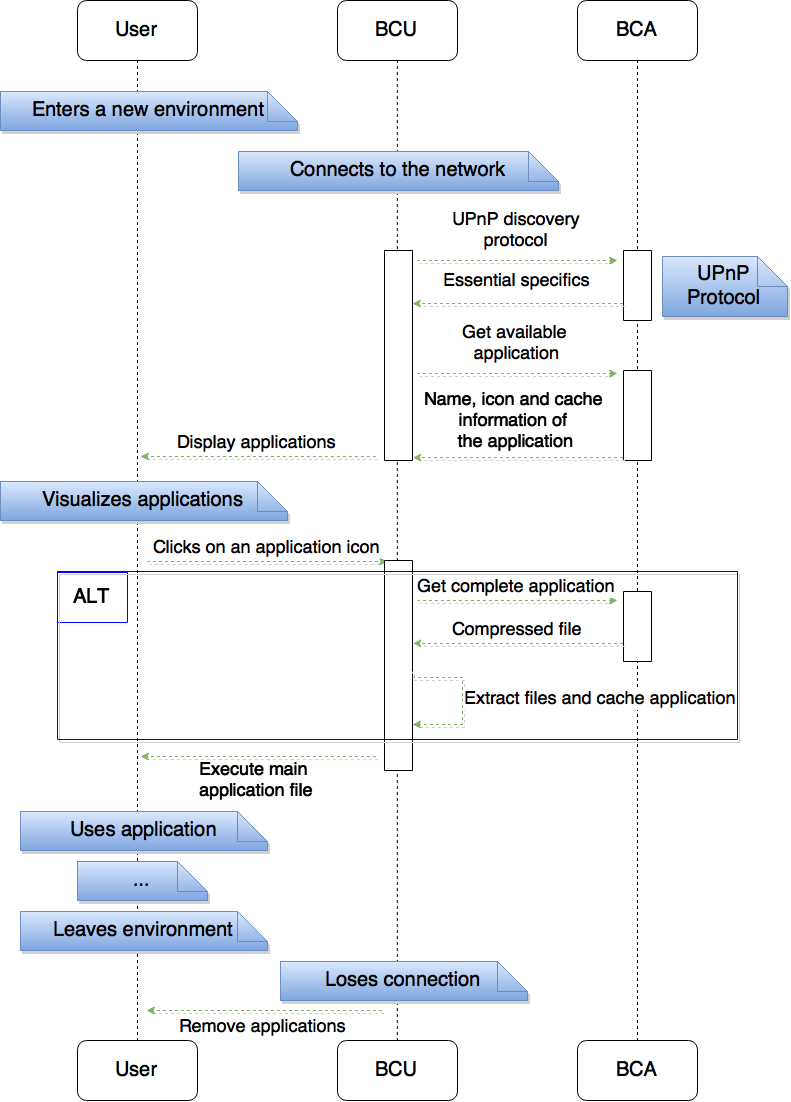
\includegraphics[width = 8.5cm, height = 8.5cm]{FIG4}
    \caption{Detailed sequence of requests exchanged by BCU and BCA.}
\end{figure}

\begin{figure}[!htb]
    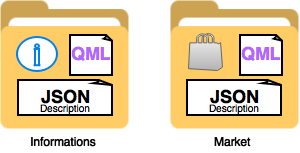
\includegraphics[scale = 0.83]{FIG3}
    \caption{Directory structure of a BCA that hosts two applications.}
\end{figure}

Consider that the application's purpose is to allow users to get information about the stores, buy itens, look for hot sales etc. By selecting the available application, the user can perform many actions inside the shopping without the need of walking through the stores. The only thing (s)he needs to do is to choose the right application and to execute it. For instance, if the user wants to buy a wallet, (s)he opens the store's  application and chooses the wallet (s)he wants. Thus, when (s)he decides to buy the wallet, the user can pay for the wallet with the store's application and get the wallet at the physical store. This kind of applications can reduce the total time that a user will take for performing his/her daily actions. Therefore, it avoids spending more time then needed. When the user leaves the environment (e.g. the shopping mall), the application is automatically deleted from his/her mobile device.

\section{Conclusion}
In this paper, we proposed a middleware for context-aware self-installable applications based on the UPnP technology, which is a wide-spread networking technology considered as being the leading technology for discovery and control of networked devices \cite{sherwin2009upnp} by the International Organization for Standardization and the International Electrotechnical Commission. In short, the proposed solution allows applications to be  installed in the main menu of the users' mobile devices without any intervention from the users and/or boring installation process, promoting the Weiser's vision of the transparent technologies for pervasive scenarios. Therefore, the proposed middleware can improve the user's experiences on using mobile services, avoiding the traditional process of searching and installing applications manually. In some cases, the user does not even know about the existence of a certain application to use in a given place. Thus, the proposed middleware can be used to expose useful services in any environments.

\ifCLASSOPTIONcaptionsoff
  \newpage
\fi 

\bibliography{references}{}
\bibliographystyle{plain}

\end{document}


